\documentclass{jsarticle}

 \usepackage{ascmac}
 \usepackage{graphicx}
 \usepackage[dvipdfmx]{color}
 \usepackage{amssymb,amsmath,amsthm}
 \usepackage{graphics}
 \usepackage{fancybox, tcolorbox}
 \tcbuselibrary{raster,skins, breakable}
 \usepackage{nccmath}
 \usepackage{tikz}
 \usetikzlibrary{intersections, calc, cd}
 \usepackage{bm}
 \usepackage[italicdiff]{physics}
 \usepackage{titlesec}
 \usepackage{mathtools}
 \usepackage{enumerate}
 \usepackage{float}

 \newcommand{\myproof}[1]{
  \begin{tcolorbox}[
    empty,top = -2pt, breakable = true,
    underlay = {
      \draw[line width = 5pt, color = teal] (frame.north west) -- (frame.south west);
      },
    underlay unbroken = {
      \fill (frame.south east) -- ([xshift = -5pt]frame.south east) --([xshift = -5pt, yshift = -7pt]frame.south east) -- ([yshift = -7pt]frame.south east) -- cycle;
    },
    underlay last = {
        \fill (frame.south east) -- ([xshift = -5pt]frame.south east) --([xshift = -5pt, yshift = -7pt]frame.south east) -- ([yshift = -7pt]frame.south east) -- cycle;
      }
    ]
    {\it Proof.}

    {#1}
  \end{tcolorbox}
 }

 \numberwithin{equation}{section}
 \setcounter{tocdepth}{3}

\theoremstyle{definition}
\newtheorem{dfn}{定義}[section]
\newtheorem{exa}{例}[section]
\newtheorem{thm}[dfn]{定理}
\newtheorem{prop}[dfn]{命題}
\newtheorem{note}[dfn]{注意}
\newtheorem{prob}[dfn]{問}
\newtheorem{coro}[dfn]{系}


\usepackage{fancyhdr}
\pagestyle{fancy}
    \lfoot{}
    \cfoot{\thepage}
    \rfoot{}

\begin{document}
\section{variance sum rule}
以後,セクション番号は論文のものを合わせてあります.
\subsection{A. derivation}
overdamped Langevin方程式は
\begin{equation}
  \dot{x}(t) = \mu F(t) + \sqrt{2D} \eta(t)
\end{equation}
であり,これを$0 \to t$で積分すれば
\begin{equation}
  x(t) - x(0) = \mu \int_0^t F(s) ds + \sqrt{2D} \int_0^t \eta(s)ds
\end{equation}
\begin{equation}
  \label{13}
  \Delta x(t) - \mu \int_0^t F(s) ds = \sqrt{2D} \int_0^t \eta(s)ds 
\end{equation}
両辺2乗すれば,
\begin{equation}
  \qty{ \Delta x(t) } ^2 + \mu^2 \qty{\Sigma_F (t)} ^2 - 2\mu \Delta x(t) \int_0^t F(s) ds = 2D \int_0^t \int_0^t \eta(s) \eta(s') dsds'
\end{equation}
\begin{equation}
  \label{15}
  \qty{ \Delta x(t) } ^2 + \mu^2 \qty{\Sigma_F (t)} ^2 = 2\mu \Delta x(t) \int_0^t F(s) ds + 2Dt
\end{equation}
となる.
ここで $C_{xF} (s) - C_{Fx} (s)$を計算しておく.
\begin{equation}
  C_{xF} (s) - C_{Fx} (s) = \langle x(s)F(0) \rangle - \langle F(s)x(0) \rangle
\end{equation}
また,$\Delta x(t), \Sigma_F (t)$に関する分散は
\begin{equation}
  \mathcal{V} _{\Delta x} (t) = \langle \qty{ \Delta x(t) } ^2 \rangle - \langle \Delta x(t) \rangle^2
\end{equation}
\begin{equation}
  \mathcal{V} _{\Sigma_F} (t) = \langle \qty{ \Sigma_F (t) } ^2 \rangle - \langle \Sigma_F (t) \rangle^2
\end{equation}
である.ここで (S4) の右辺の第2項は\footnote{以後,S4などは論文中の式番号です.}
\begin{equation}
  2 \mu \int_0^t ds \qty{ C_{xF} (s) - C_{Fx} (s) } = 2 \mu \int_0^t ds \qty{ \langle x(s)F(0) \rangle - \langle F(s)x(0) \rangle }
\end{equation}
であり,式 (\ref{15}) の右辺第1項は
\begin{align}
  2\mu \int_0^t F(s) \Delta x(t) ds &= 2\mu \int_0^t F(s) (x(t) - x(0)) ds \\
  &=2\mu \int_0^t x(t)F(s) ds - 2\mu \int_0^t x(0) F(s) ds 
\end{align}
となる.ここで式 (\ref{15}) の両辺についてアンサンブル平均をとる.このとき,先ほど示した分散の定義に注意して,
\begin{equation}
  \label{12}
  \mathcal{V} _{\Delta x} (t) + \langle \Delta x(t) \rangle^2 + \mu^2 \mathcal{V} _{\Sigma_F} (t) + \mu^2 \langle \Sigma_F (t) \rangle^2 = 2Dt + 2\mu \int_0^t \langle x(t)F(s) \rangle  ds - 2\mu \int_0^t \langle x(0) F(s) \rangle ds
\end{equation}
この右辺第2項の積分について考える.(S4)の右辺に出てくる積分を,つぎのように積分変数を$s' = t - s$として変形すれば,
\begin{align}
  2\mu \int_0^t \langle x(s)F(0) \rangle  ds &= 2\mu \int_t^0 \langle x(t - s')F(0) \rangle  (-ds') \\
  &= 2\mu \int_0^t \langle x(t)F(s') \rangle ds' \quad \text{(相関関数は時刻をずらしてもよいため)} \\
  &= 2\mu \int_0^t \langle x(t)F(s) \rangle ds
\end{align}
となり,式 (12) 第2項の積分と一致する.さらに,式 (\ref{13}) の両辺にアンサンブル平均をとれば,$\eta(t)$ が $0$になるために
\begin{equation}
  \langle \Delta x(t) \rangle - \mu \langle \Sigma_F (t) \rangle = 0
\end{equation}
\begin{equation}
  \langle \Delta x(t) \rangle^2 = \mu^2 \langle \Sigma_F (t) \rangle^2
\end{equation}
NESSを考えているので,
\begin{equation}
  \langle \Delta x(t) \rangle = \langle \Delta x(0) \rangle = 0
\end{equation}
となる.以上を考えると,式 (\ref{12}) は
\begin{equation}
  \mathcal{V} _{\Delta x} (t) + \mu^2 \mathcal{V} _{\Sigma_F} (t) = 2Dt + 2\mu \int_0^t \langle x(s)F(0) \rangle  ds - 2\mu \int_0^t \langle x(0) F(s) \rangle ds
\end{equation}
\begin{equation}
  \label{120}
  \mathcal{V} _{\Delta x} (t) + \mu^2 \mathcal{V} _{\Sigma_F} (t) = 2Dt + 2\mu \int_0^t ds ( C_{xF} (s) - C_{Fx} (s) )
\end{equation}
となる.論文では右辺第2項を $\mathcal{S} (t)$ とおき,
\begin{equation}
  \label{1}
  \mathcal{V} _{\Delta x} (t) + \mu^2 \mathcal{V} _{\Sigma_F} (t) = 2Dt + \mathcal{S} (t)
\end{equation}
\begin{equation}
  \mathcal{S} (t) := 2\mu \int_0^t ds ( C_{xF} (s) - C_{Fx} (s) )
\end{equation}
のようにまとめてある.

\section{entropy production rate}
overdamped Langevin方程式において熱はつぎのように定義される.
\begin{equation}
  d \hat{Q} := - \frac{\partial U}{\partial x} \circ  d \hat{x} 
\end{equation}
ただし $\hat{\cdot}$ のように,確率変数についてはハットをつける.また,$\circ $は Stratonovich 積を表す.
論文中では,$F$を$- \frac{\partial U}{\partial x}$と仮定しているため,エントロピー生成は
\begin{equation}
  \sigma dt = \frac{1}{k_B T} \langle F(t) \circ dx(t) \rangle
\end{equation}
となる.Stratonovich 積の定義より
\begin{align}
  \langle F(t) \circ dx(t) \rangle &= \frac{1}{2} \langle \qty{ F(t + dt) + F(t) } \qty{ x(t + dt) - x(t) } \rangle \\
  &= \frac{1}{2} \langle \qty{ F(t + dt) + F(t) } \qty{ y(t + dt) - y(t) + vdt } \rangle \quad \text{(y(t) = x(t) - vtを用いた)}
\end{align}
となる.ここでつぎの量を考える.
\begin{equation}
  C_{yF}(dt) - C_{Fy} (dt) = \langle y(dt)F(0) \rangle - \langle y(0)F(dt) \rangle
\end{equation}
また,相関関数なので
\begin{equation}
  C_{yF}(dt) - C_{Fy} (dt) = C_{yF}(t + dt) - C_{Fy} (t + dt)
\end{equation}
にも注意しておく.そうすれば,$\langle F(t) \circ dx(t) \rangle$は
\begin{align}
  \langle F(t) \circ dx(t) \rangle &= \frac{1}{2} \langle \qty{ F(t + dt)y(t + dt) - F(t)y(t)} + \qty{ F(t + dt)vdt + F(t)vdt} + \qty{ F(t)y(t + dt) - F(t + dt)y(t) } \rangle \\
  &= \frac{1}{2} \qty[ C_{yF}(dt) - C_{Fy} (dt) ] + \frac{1}{2} \cdot 2 \langle F(t) \rangle vdt \\
  &= \frac{1}{2} \qty[ C_{yF}(dt) - C_{Fy} (dt) ] + \frac{v^2}{\mu } dt \quad \quad (\because \langle F(t) \rangle = \frac{v}{\mu })
\end{align}
となり,S13を得た.これをTaylor展開する.
\begin{align}
  \langle F(t) \circ dx(t) \rangle &= \frac{1}{2} \qty[ \qty( C_{yF}(0) + \dot{C}_{yF}dt + \cdots ) - \qty( C_{Fy}(0) + \dot{C}_{Fy}dt + \cdots  ) ] + \frac{v^2}{\mu } dt \\
  &= \frac{1}{2} \qty[ \dot{C}_{yF} - \dot{C}_{Fy} ] + \frac{v^2}{\mu } dt
\end{align}
$D=k_B T \mu$に注意して,$\sigma $の表式に戻せば
\begin{equation}
  \label{s15}
  \sigma|_{t = 0} = \frac{1}{2k_B T} \qty[ \dot{C}_{yF} - \dot{C}_{Fy} ] + \frac{v^2}{D}
\end{equation}
となり,$\mathcal{S} (t) $を用いて書くと
\begin{equation}
  \sigma = \frac{1}{4D} \frac{\partial^2}{\partial t^2} \mathcal{S} (t) |_{t = 0}  + \frac{v^2}{D}
\end{equation}
となる.これがS16.

\subsection{A. entropy production from the VSR}
式 (\ref{120}) の両辺を $D( =k_B T \mu )$ で割る.
\begin{equation}
  \mathcal{V} _{\Delta x} (t) + \mu^2 \mathcal{V} _{\Sigma_F} (t) = 2Dt + 2\mu \int_0^t ds ( C_{xF} (s) - C_{Fx} (s) )
\end{equation}
\begin{equation}
  \therefore \quad \frac{1}{k_B T} \qty( \frac{1}{\mu} \mathcal{V} _{\Delta x} (t) + \mu \mathcal{V} _{\Sigma_F} (t)) = 2t + \frac{2}{k_B T} \int_0^t ds ( C_{xF} (s) - C_{Fx} (s) )
\end{equation}
両辺を2回微分して,$t=0$を考える.
\begin{equation}
  \frac{1}{k_B T} \qty( \frac{1}{\mu} \frac{\partial^2}{\partial t^2} \mathcal{V} _{\Delta x} (t) + \mu \frac{\partial^2}{\partial t^2} \mathcal{V} _{\Sigma_F} (t)) = \frac{2}{k_B T} ( \dot{C_{xF}} (t) - \dot{C_{Fx}} (t) ) \quad \text{for \ t = 0}
\end{equation}
ここで
\begin{equation}
  \frac{\partial^2}{\partial t^2} \mathcal{V} _{\Sigma_F} (t)|_{t = 0} = 2 \mathcal{V}_F (0)
\end{equation}
と,式 (\ref{s15}) を用いて 
\begin{equation}
  \sigma = \frac{v^2}{D} + \frac{1}{k_B T} \qty( \frac{1}{4 \mu } \frac{\partial^2}{\partial t^2} \mathcal{V} _{\Delta x} (t)|_{t = 0} + \frac{\mu }{2} \mathcal{V}_F (0) )
\end{equation}

\section{optically trapped bead dragged through water}
overdamped Langevin方程式 
\begin{equation}
  \dot{x} (t) = \mu F(t) + \sqrt{2D} \eta (t)
\end{equation}
に $y(t) = x(t) -vt$ と $F(t) = k(vt - x)$ を代入して
\begin{equation}
  \dot{y}(t) + v = \mu k (vt - y(t) - vt) + \sqrt{2D} \eta(t)
\end{equation}
$\mu = \gamma^{-1}$ を使って
\begin{equation}
  \label{s21}
  \gamma \dot{y} (t) = -k y(t) - \gamma v + \sqrt{2 k_B T \gamma } \eta(t)
\end{equation}
となり,これが (S21).\\
$y(t) = x(t) -vt$ であることより,$y(t)$ と$x(t)$には定数のずれしかないので
\begin{equation}
  \mathcal{V}_{\Delta x} (t) = \mathcal{V}_{\Delta y} (t)
\end{equation}
が分かり,式 (\ref{s21}) より
\begin{equation}
  \mathcal{V}_{\Delta y} (t) = \frac{2 k_B T}{k} \qty( 1 - e^{-\frac{t}{\tau_r}} )
\end{equation}
が計算により求まる.ただし
\begin{equation}
  \gamma = 6 \pi \nu R, \quad \langle \eta(t) \eta(s) \rangle = \delta (t-s), \quad \tau_r := \frac{\gamma}{k}
\end{equation}
を用いた.また,
\begin{equation}
  \mathcal{V}_{\Sigma F} (t) = 2 k_B T \gamma \qty( t - \tau_r \qty( 1 - e^{-\frac{t}{\tau_r}} ) )
\end{equation}
も計算できる.以上の結果を用いて
\begin{equation}
  \mathcal{V}_{\Delta x} (t) + \mu^2 \mathcal{V}_{\Sigma F} (t) = 2Dt 
\end{equation}
と計算でき,
\begin{equation}
  \mathcal{S} (t) = 0 
\end{equation}
と分かり,エントロピー生成は
\begin{equation}
  \sigma = \gamma v^2
\end{equation}
と計算できる.

\section{Reversed thermosynamic uncertainly relation}
$\mathcal{S} (t) = 0 $であるとき,式 (\ref{vsr1})から,
\begin{equation}
  \mathcal{V}_{\Delta x} (t) \leqslant 2Dt 
\end{equation}
\begin{equation}
  \mathcal{V}_{\Sigma F} (t) \leqslant \frac{2D}{\mu ^2} t 
\end{equation}
が分かる.もちろん $\mathcal{S} (t) \neq  0 $ のときは,成り立たない.\\
\quad ここで光ピンセットからビーズに行う仕事
\begin{equation}
  W(t) = v \Sigma _F (t) = v \int_0^t ds F(s)
\end{equation}
の分散 $\mathcal{V}_{W} (t)$ を用いて,不等式を書き直すことを考える.すぐ上の定義より
\begin{equation}
  \mathcal{V}_{W} (t) = v \mathcal{V}_{\Sigma F} (t)
\end{equation}
なので,
\begin{equation}
  \frac{\mathcal{V}_{W} (t)}{v^2} \leqslant \frac{2D}{\mu^2} t 
\end{equation}
\begin{equation}
  \frac{\mathcal{V}_{W} (t)}{v^2 \gamma^2} \leqslant 2Dt 
\end{equation}
さらに,
\begin{equation}
  \langle W(t) \rangle = \gamma v^2 t = \sigma t 
\end{equation}
を用いて
\begin{equation}
  \frac{\mathcal{V}_{W} (t)}{v^2 \gamma^2} \leqslant 2Dt  = 2 k_B T t \frac{1}{\gamma}
\end{equation}
\begin{equation}
  \therefore \quad \frac{\sigma }{k_B T} \leqslant \frac{2 \langle W(t) \rangle^2}{t \mathcal{V}_{W} (t)}
\end{equation}
と書き直せる.これが (S24).

\section{Stochastic switching trap (SST)}
行間の説明のみをメモ程度に書きます(時間があるときに丁寧な説明に書きなおします).\\
\quad (S25) のアンサンブル平均を取ると,$\langle \dot{x}(t) \rangle = 0$,$q := \langle \theta (t)\rangle$,$\langle \eta (t) \rangle = 0$ より
\begin{equation}
  \langle x(t) \rangle = q \Delta \lambda
\end{equation}
となる.\\
\quad (S25)を離散化すると,(S26a), (S26b)になる.(S26b)が,論文のようになることがまだ理解できていない.\\
\quad (S26a) に $x(0)$ をかけて,
\begin{equation}
  x(t + dt)x(0) = x(t)x(0) - w_r x(t) x(0) dt + \mu k \Delta \lambda \theta (t) x(0) dt + \sqrt{2 k_B T \mu } x(0) d \mathfrak{B}_t^x  
\end{equation}
アンサンブル平均をとれば
\begin{equation}
  C_{xx} (t + dt) - C_{xx} (t) = - w_r C_{xx}(t) dt + \mu k \Delta \lambda C_{\theta x} (t) dt 
\end{equation}
両辺を $dt$ で割って,$dt \to 0$
\begin{equation}
  \frac{\partial }{\partial t} C_{xx} (t) = -w_r C_{xx} (t) + \mu k \Delta \lambda C_{theta x} (t) 
\end{equation}
これが (S27a).同様に(S26a)に$\theta (0)$をかけて,アンサンブル平均をとれば,(S27b)になる.\\
\quad (27c), (S27d) がまだ理解できていない.これら以外の行間については,(S33)までは代入して計算するだけ.

\section{Reduced VSR }
見えない自由度がある場合であっても,Reduced VSR を用いることで,$x(t)$ のみの情報から解析することができる.しかし,読んでいくと分かるように,実際には測定することのできない力 $F^I (t)$ は,測定できる変数 $x(t)$に依存しないことと,$F^I (t)$の時間相関を知っていなければ解析することはできない.\\
\quad まずは論文のように,プローブ粒子に対して線形な力 $-kx(t) $ と,測定できない力 $F^I (t)$がかかっている場合を考える.すなわち,$F(t) = -kx(t) + F^I (t)$ を (S1) に代入して,
\begin{equation}
  \dot{x} (t) + k \mu x(t) = \mu F^I (t) + \sqrt{2D} \eta (t)
\end{equation}
これが(S34).ここから,これまでと同様の方法で分散についての式を得る.\\
\quad まずは $0 \to t$ で積分し,見やすさのため文字で置き換える.
\begin{equation}
  \Delta x(t) + k \mu \int_0^t x(s) ds = \mu \int_0^t F^I (s) ds + \sqrt{2D} \int_0^t \eta(s) ds 
\end{equation}
\begin{equation}
  \Delta x(t) + k \mu \Sigma_x (t) = \mu \Sigma_{F^I} (t) + \sqrt{2D} \int_0^t \eta(s) ds 
\end{equation}
両辺を2乗して,
\begin{equation}
  \label{nizyo}
  \qty{\Delta x(t)}^2 + 2 \qty{\Delta x(t)} \mu k \Sigma_x (t) + k^2 \mu^2 \qty{\Sigma_x (t)}^2 = \mu^2 \qty{\Sigma_{F^I} (t) }^2 + 2D \int_0^t ds \int_0^t ds' \eta(s) \eta(s') + 2 \sqrt{2D} \mu \Sigma_{F^I} (t) \int_0^t \eta (s) ds 
\end{equation}
上の式を変形して(S35)にするために,先にいくつかの量について,計算しておく.
\begin{equation}
  \label{zyoken1}
  \langle \qty{\Delta x(t)}^2 \rangle = \mathcal{V} _{\Delta x} (t) + \langle \Delta x(t) \rangle ^2 = \mathcal{V} _{\Delta x} (t)
\end{equation}
\begin{equation}
  \langle \qty{\Sigma_x (t)}^2 \rangle = \mathcal{V} _{\Sigma_x} (t) + \langle \Sigma_x (t) \rangle ^2 {=} \mathcal{V} _{\Sigma_x} (t) 
\end{equation}
\begin{equation}
  2D \int_0^t ds \int_0^t ds' \eta(s) \eta(s') = 2Dt 
\end{equation}
\begin{equation}
  C_{F^I F^I} (u) = \langle F^I (u) F^I (0) \rangle - \langle F^I (0) F^I (0) \rangle = \langle F^I (u) F^I (0) \rangle
\end{equation}
つぎに
\begin{equation}
  \int_0^t ds \int_0^t du \langle F(s) F(u) \rangle = 2 \int_0^t ds \int_0^s du \langle F(y) F(0) \rangle
\end{equation}
を示す.
\begin{align}
  (\text{左辺}) &= \int_0^t ds \int_0^t du \langle F(s-u) F(0) \rangle \quad (\because \text{相関関数は時刻をずらせる}) \\
  &= \int_0^t ds \int_s^{s-t} (-dy) \langle F(y) F(0) \rangle \quad (y = s - u) \\
  &= \int_0^t ds \int_{s-t}^s dy \langle F(y) F(0) \rangle
\end{align}
これで示すべきは
\begin{equation}
  \int_0^t ds \int_{s-t}^s dy \langle F(y) F(0) \rangle = 2 \int_0^t ds \int_0^s dy \langle F(y) F(0) \rangle
\end{equation}
になった.これは下図を参考にすればよい.しかし,$y = 0$より上の領域と,下の領域で相関関数が同じ振る舞いをするとは限らないことに注意.ここについては上手く示せていない.

\begin{figure}[H]
  \begin{center}  
  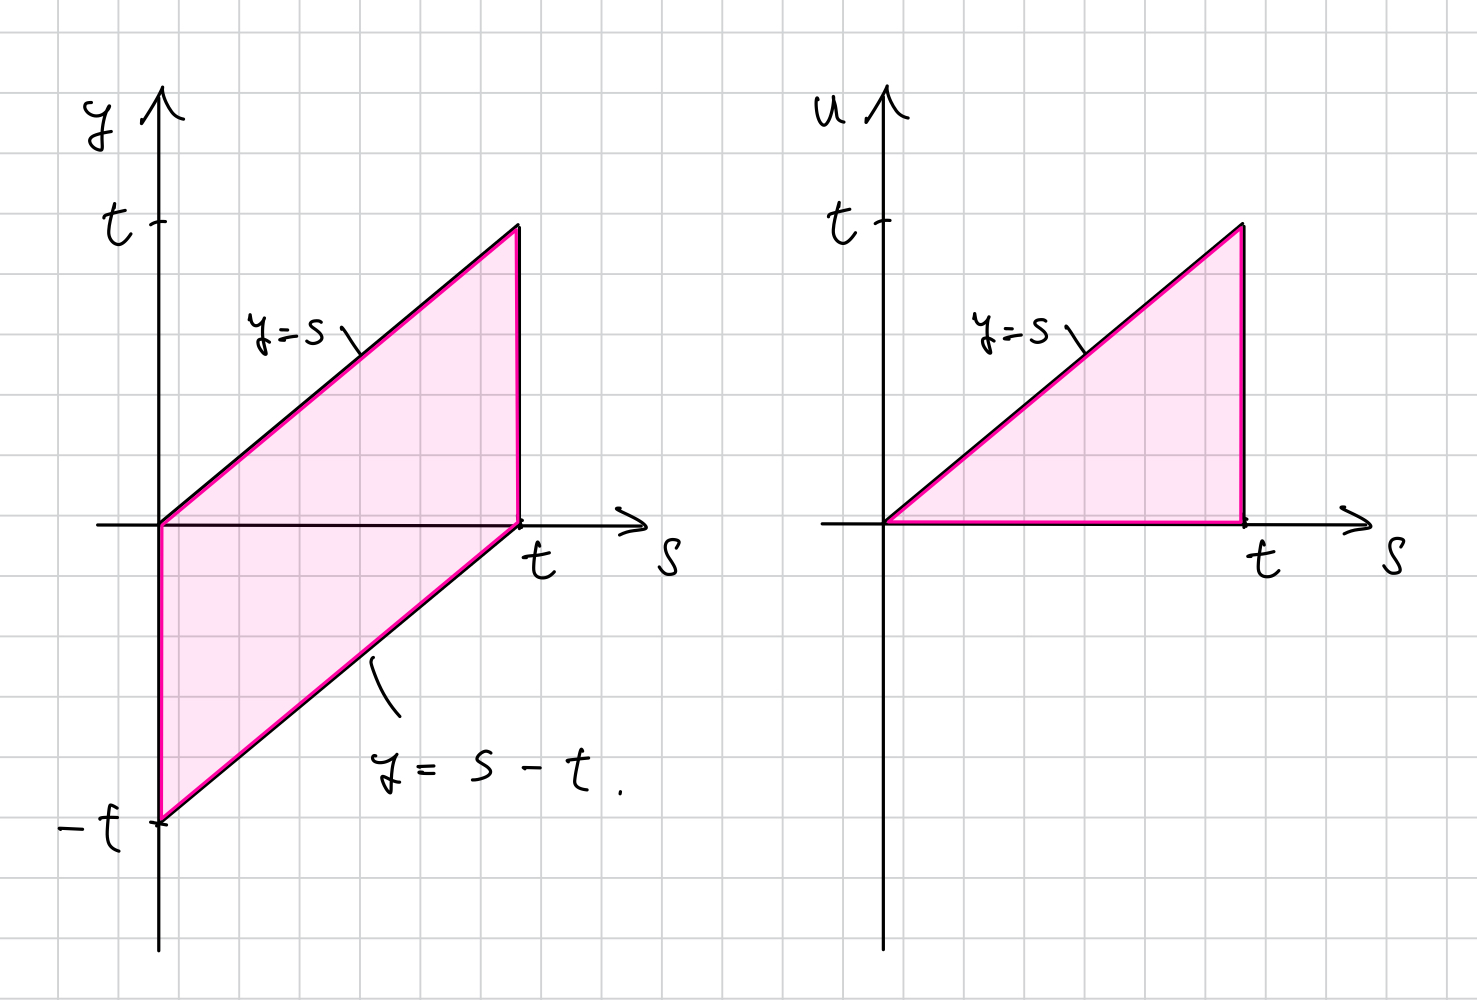
\includegraphics[width=10cm]{int_inv.jpg}  
  \end{center}
\end{figure}

最後に
\begin{equation}
  \qty{\Delta x(t)} \mu k \Sigma_x (t) = 0
\end{equation}
を示す.
\begin{align}
  \Delta x(t) \Sigma_x (t) &=   \Delta x(t) \int_0^t x(s) ds \\
  &= \int_0^t x(t)x(0) ds - \int_0^t x(0) x(s) ds 
\end{align}
であって,
\begin{align}
  \int_0^t x(0) x(s) ds &= \int_t^0 x(0)x(t-s') ds' \quad (s' = t-s) \\
  &= \int_0^t x(0) x(t-s') ds' \\
  &= \int_0^t x(s') x(t) ds'
\end{align}
となるため,
\begin{equation}
  \Delta x(t) \Sigma_x (t) = \int_0^t x(t)x(0) ds - \int_0^t x(0) x(s) ds = 0
\end{equation}
となる.\\
\quad 式 (\ref{nizyo}) に 式 (\ref{zyoken1}) からの関係式を代入することで,次を得る.
\begin{equation}
  \mathcal{V} _{\Delta x} (t) + \mu^2 k^2 \mathcal{V} _{\Sigma_x} (t) = 2Dt + 2\mu^2 \int_0^t ds \int_0^s du C_{F^I F^I} (u) + 4\mu \sqrt{2D} \int_0^t ds \int_0^s du C_{F^I \eta } (u)   
\end{equation}
となる.これは (S36) の最後の項の係数が2倍だけずれている.\\
論文ではここから,測定することのできない力 $F^I (t)$ が測定できる変数 $x(t)$に依存しないことと,$F^I (t)$の時間相関の具体的な表式を与えることで,実験により求められるように変形している.なお,ここでの仮定により,先ほどの2倍のズレは関係ない. \\

\newpage 
\section{RBC MODEL}
ここでは Reduced VSR をヒト赤血球(RBC)に適用する.RBCは解糖系を通してグルコースをATPに代謝し,細胞膜のアクティブな振動を引き起こし,それに伴いエントロピーが生成する.\par 
この論文では3つの方法でRBCの実験を行った.1つは異なる強度の光トラップにより,膜に非特異的に結合したビーズを使ってRBCを機械的に引き延ばす方法.2つ目は先行研究(11)のデータを用いてRBC膜を機会的にセンシングする方法.3つ目は振動セグメントの追跡により,膜の輪郭の揺らぎを測定する方法である.\par 
ここでは figure S1 のように,見えない変数 $y(t)$ を設定した2層モデルを検討した.$x(t)$は測定することができる変数である.これらの変数はつぎの方程式を満たす.
\begin{equation}
  \dot{x}(t) = \mu_x (-k_b x(t) - k_{int}(x(t) - y(t)) + C_1) + \sqrt{2D_x} \eta^x (t) 
\end{equation}
\begin{equation}
  \dot{y}(t) = \mu_y (-k_c y(t) + k_{int}(x(t) - y(t)) + f^a (t) + C_2) + \sqrt{2D_y} \eta^y (t) 
\end{equation}
ここで $k_{i}$ は実効的な力の定数であり,$\mu_{i}, \eta_{i}$は移動度とホワイトノイズである.また,$C_i$は定数,$D_i$は $D_i = k_B T \mu_i$ である.$f^a (t)$は確率的なアクティブ力であって,つぎの関係を満たす.
\begin{equation}
  \dot{f}^a (t) = - \frac{f^a (t)}{\tau_a} + \sqrt{\frac{2 \epsilon^2}{\tau_a}} \eta^f (t)
\end{equation}



\end{document}